\section{Results}

\subsection{DrawAFriend Game Statistics}

After months in smaller-scale trials, DrawAFriend was released publicly on January 8th, 2013. Our player recruitment strategy was very successful: by Jaunuary 11th players had downloaded the game over 2000 times and created 6373 drawings. In total, players had spent just under 10 full 24 hour days drawing.

Players were given the option of drawing Facebook friends or one of an initial set of six celebrities: Robert Downey Jr., Angelina Jolie, Kim Kardashian, Barack Obama, Brad Pitt, or Kristen Stewart. From the drawings generated in the first four days, we manually chose 611 celebrity drawings to be used for analysis. The statistics in Figure \ref{fig:daf-stats} reference the 611 drawings.

\begin{figure}[b]
  \centering%
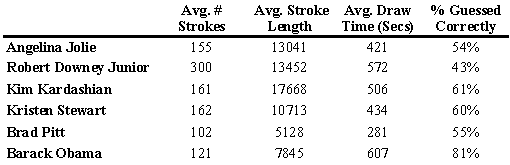
\includegraphics[height=1.1in]{./figures/daf-stats-cropped.pdf}
  \caption{Celebrity drawing statistics for 611 hand-picked drawings from the first four days after launch.}
  \label{fig:daf-stats}
\end{figure}

We ran our modified mean shift algorithm on this initial dataset to create the correction vector fields shown in Figure \ref{fig:image-table}. Our MATLAB implementation took under 5 minutes for each celebrity. The great majority of the time was spent in un-optimized nearest neighbor search.

\subsection {Drawing Enhancements}

We applied the correction vector field to interactively modify strokes during the drawing process (see accompanying video). With no additional user interface elements to the existing DrawAFriend UI, we seamlessly added stroke auto-correction. As the user draws, strokes are subtly corrected at interactive rates on an iPhone 4. In general, the fact that corrections are being applied is almost invisible to the user. Instead, strokes appear where the user {\em intended} to draw.

%????Please see the \alex{Not sure how to reference the teaser on top} and the video for interactive examples.

We also applied the correction vector field retrospectively to improve the existing database of user drawings. The drawings are already quite good, making the corrections made by the vector field all the more impressive.  While the algorithm universally improves the images by making the celebrity far more recognizable, it does so without sacrificing style. For comparisons of the raw drawings and the corrected images please see our video and the supplementary website.

\begin{figure}
\centering
\begin{tabular}{ccccc}
\imgtbl{image_aj} & \imgtbl{avg_aj} & \imgtbl{dir_aj} & \imgtbl{mag_aj} & \imgtbl{edges_aj} \\
\imgtbl{image_bp} & \imgtbl{avg_bp} & \imgtbl{dir_bp} & \imgtbl{mag_bp} & \imgtbl{edges_bp} \\
\imgtbl{image_kk} & \imgtbl{avg_kk} & \imgtbl{dir_kk} & \imgtbl{mag_kk} & \imgtbl{edges_kk} \\
\imgtbl{image_ks} & \imgtbl{avg_ks} & \imgtbl{dir_ks} & \imgtbl{mag_ks} & \imgtbl{edges_ks} \\
\imgtbl{image_rd} & \imgtbl{avg_rd} & \imgtbl{dir_rd} & \imgtbl{mag_rd} & \imgtbl{edges_rd} \\
\imgtbl{image_bo} & \imgtbl{avg_bo} & \imgtbl{dir_bo} & \imgtbl{mag_bo} & \imgtbl{edges_bo} \\
(a) & (b) & (c) & (d) & (e)
\end{tabular}
\caption{DrawAFriend users draw one of six celebrities (a). We use our database of hundreds of drawings per subject -- shown averaged in (b) -- to precompute a \emph{correction vector field} (c) enabling real-time drawing assistance on the iPhone. The magnitude of our vector field (d) reveals a consensus of artistic renderings strikingly different than what we could compute with automated methods, such as a canny edge detector (e).}
\label{fig:image-table}
\end{figure}
